Come appena visto Code Red ha costituito una vera e propria piaga, che si è propagata in ogni angolo del pianeta e ha causato gravi danni nonostante sia stato scoperto diversi giorni prima che la seconda versione facesse la sua comparsa ed iniziasse a diffondersi in modo efficace.\\
A fronte di ciò, abbiamo effettuato una simulazione per vedere cosa sarebbe accaduto se il worm non fosse stato scoperto, e quindi avere una misura dell’entità del danno in termini di numero di host compromessi, così poi da confrontare i risultati con il caso reale in cui la consapevolezza della presenza di tale minaccia ha spinto gli utenti ad adottare contromisure come patch, firewall, antivirus e simili.\\
Per fare questo, innanzitutto è stato necessario l’ausilio di un modello epidemico che simulasse fedelmente il comportamento ed in particolare la diffusione del worm.\\
I classici modelli per lo studio dello sviluppo epidemico, però, non sono adatti a replicare il comportamento di Code Red, perché non tengono conto delle contromisure umane intraprese durante il processo di diffusione e inoltre considerano il tasso di infezione costante nel tempo. Questi due fattori hanno portato Zou et al.~\cite{two-factor} alla derivazione del “Two Factor Worm Model” con cui hanno dimostrato tramite simulazione che i risultati approssimano bene l’andamento dei dati osservati, in particolare sono riusciti a giustificare il rallentamento delle scansioni che si è verificato appena prima il cessamento dell’attività di diffusione del worm. Tale evento, infatti, è la conseguenza della violenta propagazione su larga scala che ha provocato congestionamento e danni alla rete.\\
Le figure~\ref{tf_model} e~\ref{tf_compare} mostrano i risultati ottenuti da Zou et al., in particolare la figura~\ref{tf_compare} mostra il confronto con i dati reali osservati da Goldsmith and Eichman~\cite{gold, eich}.\\
\begin{figure}
    \centering
    \begin{minipage}{0.5\textwidth}
        \centering
        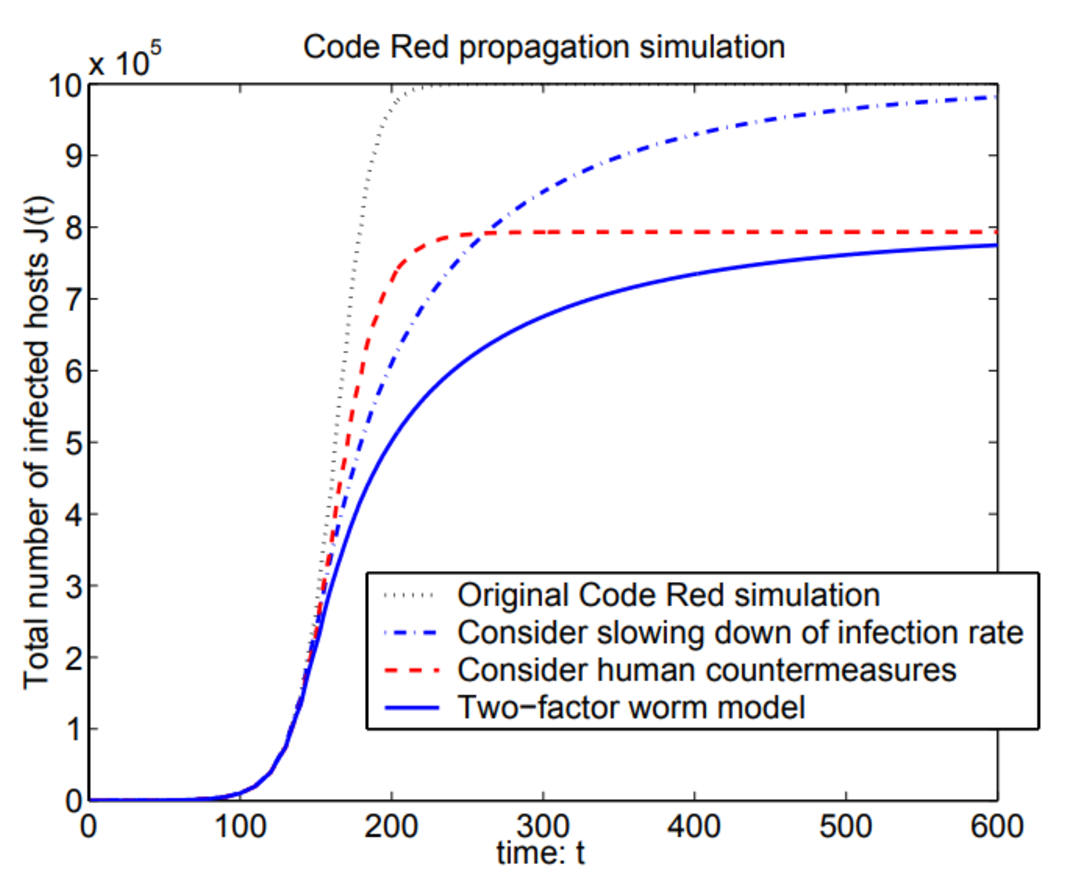
\includegraphics[width=0.95\textwidth]{images/tf_model} % first figure itself
        \caption{infezioni al variare del tempo}
        \label{tf_model}
    \end{minipage}\hfill
    \begin{minipage}{0.5\textwidth}
        \centering
        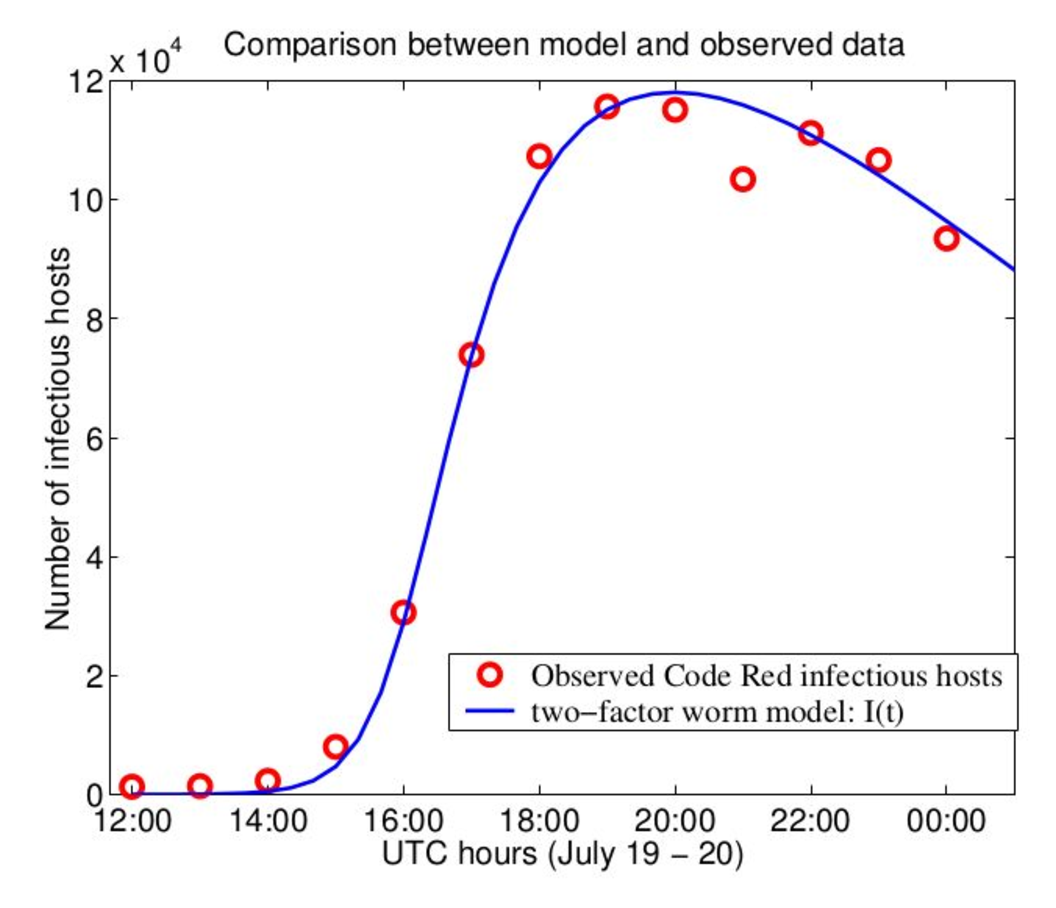
\includegraphics[width=0.95\textwidth]{images/tf_compare} % second figure itself
        \caption{confronto dati-modello}
        \label{tf_compare}
    \end{minipage}
\end{figure}
Di seguito è riportato il set di equazioni differenziali che descrivono il sistema, caratterizzanti sono il fattore $\beta(t)$ che rappresenta la frequenza di infezione variabile nel tempo, ed i fattori $R(t)$ e $Q(t)$ che costituiscono il numero di host rimossi dalla popolazione infetta a seguito di contromisure a valle del contagio, ed il numero di host rimossi dalla popolazione suscettibile (vulnerabile) a seguito di contromisure a monte, le altre variabili sono riassunte nella tabella di figura~\ref{notations}.\\
\begin{equation}
\left\{  \begin{array}{rcl} 
                dS(t)/dt &=& -\beta(t)S(t)I(t) - dQ(t)/dt, \\ 
                dR(t)/dt &=& \gamma I(t), \\ 
                dQ(t)/dt &=& \mu S(t)J(t), \\ 
                \beta(t) &=& \beta_{0}[1 - I(t)/N]^{\eta}, \\ 
                N &=& S(t) + I(t) + R(t) + Q(t), \\
                I(0) &=& I_{0} \ll N; S(0) = N -I_{0}; R(0) = Q(0) = 0; 
           \end{array}  \right.
\end{equation}
La simulazione è stata eseguita con lo stato iniziale specificato dai seguenti parametri: $N = 1000000$, $I_{0} = 1$, $\eta = 3$, $gamma = 0.05$, $\mu = 0.06/N$ , e $\beta_{0} = 0.8/N$.\\
$I_{0}$ e $\beta_{0}$ rappresentano rispettivamente numero di host infetti e tasso di infezione iniziali, $\gamma$ e $\mu$ i tassi di rimozione, infine $\eta$ è un parametro di sensibilità che regola $\beta(t)$ in funzione di $I(t)$, sostanzialmente è un fattore che indica quanto il tasso di infezione dipende dal numero di host infetti in un certo istante di tempo, ad esempio $\eta = 0$ implica un tasso di infezione costante.\\
\begin{figure}[!hbp]
\centering
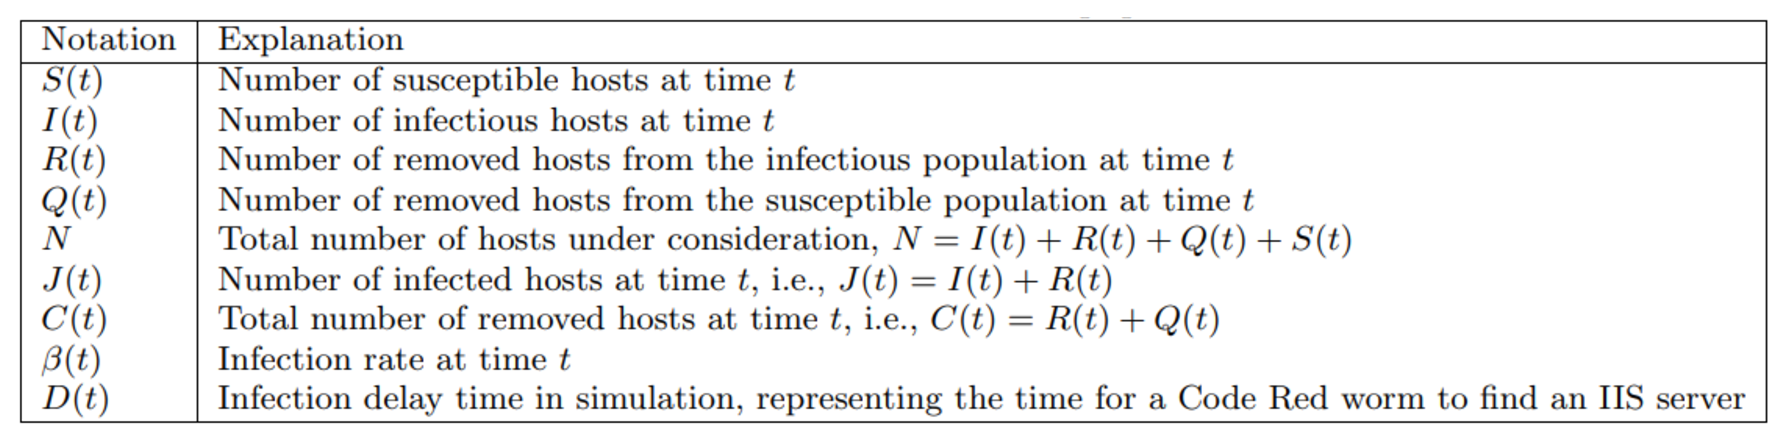
\includegraphics[width=0.95\textwidth]{images/notations.eps}
\caption{notazioni variabili del modello}
\label{notations}
\end{figure}
Il nostro studio è consistito nel semplificare il “Two Factor Model” eliminando il fattore relativo alle contromisure intraprese dagli utenti, proprio come se il worm avesse potuto agire indisturbato senza che nessuno si accorgesse della sua presenza, pertanto le variabili  R(t) e Q(t) relative agli host in stato di “rimosso” sono state annullate, ottenendo così il seguente modello semplificato:
\begin{equation}
\left\{  \begin{array}{rcl} 
                dS(t)/dt &=& -\beta(t)S(t)I(t), \\ 
                \beta(t) &=& \beta_{0}[1 - I(t)/N]^{\eta}, \\ 
                N &=& S(t) + I(t), \\
                I(0) &=& I_{0} \ll N; S(0) = N -I_{0}; 
           \end{array}  \right.
\end{equation}
La simulazione è stata realizzata tramite Simulink, a partire dalle stesse condizioni iniziali poste da Zou et al. e per un tempo di simulazione equivalente a circa 24h.\\
I risultati ottenuti (Figura~\ref{simpler}) mostrano che in 12 ore (metà tempo di simulazione) circa il 70\% degli host suscettibili sono stati infettati, approssimativamente la stessa proporzione della simulazione effettuata da Zou et al., quindi in definitiva il fatto che Code Red sia stato scoperto prima della sua violenta diffusione non ha alleviato significativamente le conseguenze in termini di macchine infettate.\\
Questo risultato mette in evidenza che di fronte ad un worm così aggressivo come Code Red, con un tasso di propagazione che ha raggiunto un picco di 2000 infezioni al minuto, le contromisure che vengono adottate a seguito dell’inizio dell’epidemia non contribuiscono a porre rimedio in maniera efficace da un punto di vista globale, ma ciò che può fare la differenza sono le contromisure preventive che vengono attuate prima degli attacchi, ovvero quelle che tendono a ridurre il numero di host potenzialmente a rischio. Quindi il vero fattore che ha favorito gli effetti devastanti del worm è stata la mancata applicazione della patch che andava ad eliminare la vulnerabilità sfruttata, nonostante fosse stata resa disponibile non poche settimane prima della comparsa della minaccia.\\
\begin{figure}[!hbp]
\centering
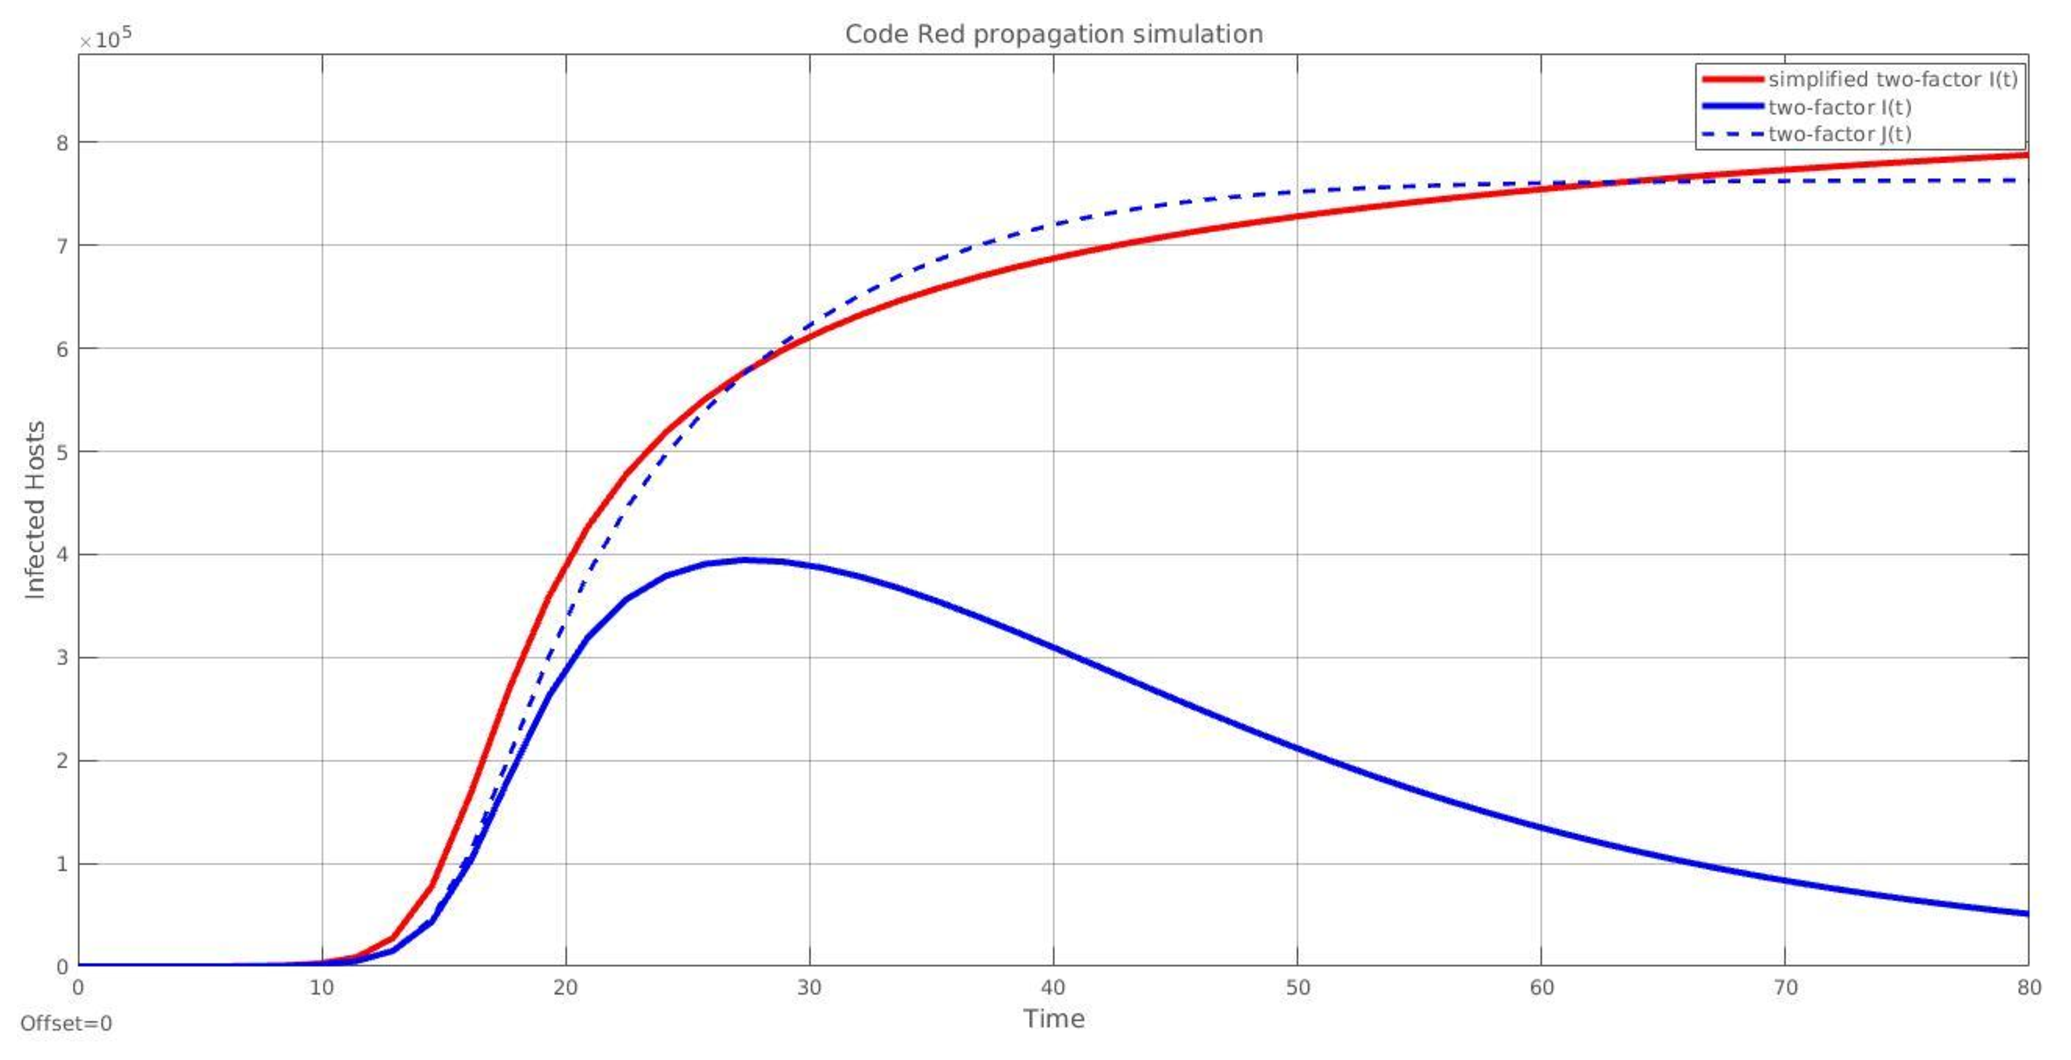
\includegraphics[width=0.95\textwidth]{images/simpler.eps}
\caption{modello semplificato vs. two-factor}
\label{simpler}
\end{figure}
